\documentclass[12pt,a4paper,titlepage]{article}

\usepackage{times}
\usepackage{setspace}
\usepackage{textcomp}
\usepackage[a4paper,left=1in,top=1in,right=1in,bottom=1in]{geometry}
\usepackage{graphicx}

\usepackage[english]{babel}
\usepackage[backend=bibtex]{biblatex}
\usepackage{csquotes}

\usepackage[bookmarks]{hyperref}
\hypersetup{colorlinks=true,allcolors=black}
\usepackage{hypcap}


\bibliography{sources}


\doublespacing{}
\oddsidemargin = 0pt
\headheight = 0pt
\topmargin = 0pt
\headsep = 0pt
\marginparwidth = 0pt
\textwidth = 450pt


\begin{document}

\title{Apple Inc.}
\author{Kevin Bloom \\ MET315--02}
\maketitle

\newpage

\pagenumbering{roman}
\tableofcontents

\newpage

\pagenumbering{arabic}

\section{Description of Company}
Apple is one of the most successful companies of all time. Not only in the
U.S. but in the whole world. They are one of the biggest designers/manufacturers
of desktops, laptops/netbooks, tablets, and smartphones as
well~\cite{hoover}. Not to mention their massive grip on the multimedia realm
with iTunes, Apple Music, Apple TV, and their assortment of multimedia editing
programs. They don't only rule the school of multimedia and are rapidly seizing
the tech world due to it's easy-to-use interface and unix-based (DarwinOS)
background. Monetarily, the company does extremely well; as would any company
among the top in the world. Just one of their products, the iPhone, is
responsible for two-thirds of the company's revenue~\cite{hoover}. This may not
be too surprising because pretty much \emph{everyone} has an iPhone! That being
said, Apple's biggest claims to fame are as a computer hardware/software
manufacturing/designing company and as a catalyst of new technology in the
market.

Mostly everyone has heard of the founders Steve Jobs and Steve Wozniak. Wozniak
left the company in 1983, only 3 years after the company went
public~\cite{hoover}. Jobs was with the company on and off\footnote{In 1985,
  Jobs resigned from Apple due to workplace drama with John Sculley. He rejoined
  Apple in 1997~\cite{jobs}.} until his death in 2011. After his death, Tim Cook
took over as CEO and remains CEO to this day. A few other notable employees of
the company are: Dr. Arthur Levinson, chairman, Jeff Williams, COO, Jonny Ive,
chief design officer, Craig Federighi, SVP software engineer, Dan Riccio, SVP
hardware engineer, and Phil Schiller, SVP worldwide marketer~\cite{hoover}. We
know most of these people from Apple's events which they come on stage to
talk. Jonny Ive is most known for the videos that reveal the newest Apple
projects. Either way, without these people, and many more, Apple would not be as
successful as it is today.

Most people know that Apple doesn't assemble most of their devices in the
US. How do they know this? Well, on the back of any Apple device, there will be
a note informing the user that it was designed in the US but assembled in
China. According to LexisNexis Academic, they have a subsidiary called
\emph{AuthenTec}. One of the locations for this company is in Shanghai, which I
believe is the main manufacturing plant for some of their bigger
products~\cite{lexis}. That being said, there are also some plants/facilities
found in Japan, Mexico, Europe, and even Australia~\cite{lexis}. Their
headquarters is located in Cupertino, Califonia and is approximately 16,000
sq. ft in size~\cite{hoover}. Apple has hundreds of locations all over the
world, ranging from design facilities to retail stores to manufacturing.

Needless to say, Apple does a lot of business. They sell a lot of product. In
fact, in 2016 they had about \$215,639,000 worth of sales~\cite{hoover}!
Also according to Hoover, they have a market value of about
\$594,339,610. Talk about big numbers! Apple sold approximately 226,200,000
iPhones~\cite{lifewire} and about 45,590,000 iPads~\cite{lifewire2} in 2016
alone. Just based on those approximate numbers, we can determine that Apple gets
all most all of it's revenue from the iPhone.\footnote{The iPhone, at full
  retail price, is about \$800. Multiply that by the number of sold iPhones, we
  get \$180,960,000. That's about 84\% of their sales!} Let's not forget the
other slew of products they sell that weren't mentioned. That being said, the
volume of product from Apple is absolutely enormous! Along with their huge fan
base, it's no wonder they are so successful.

\newpage

\section{Stock Chart}

\begin{figure}[!htb]
  \centering
  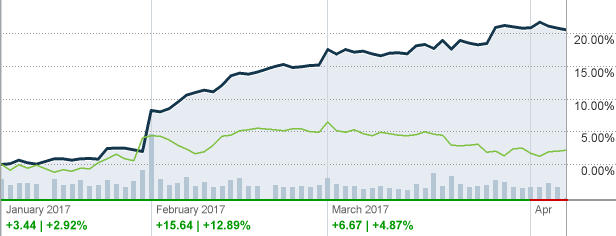
\includegraphics[width=1\textwidth]{apple-chart-3mo}
    \caption{Apple (blue) vs NASDAQ (green) for 3 months~\cite{cnnapple}}
\end{figure}


\begin{figure}[!htb]
  \centering
  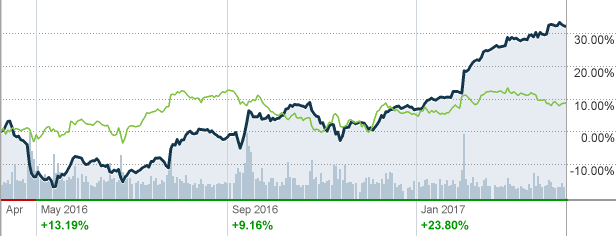
\includegraphics[width=1\textwidth]{apple-chart-1yr}
    \caption{Apple (blue) vs NASDAQ (green) for 1 year~\cite{cnnapple}}
\end{figure}

\begin{figure}[!htb]
  \centering
  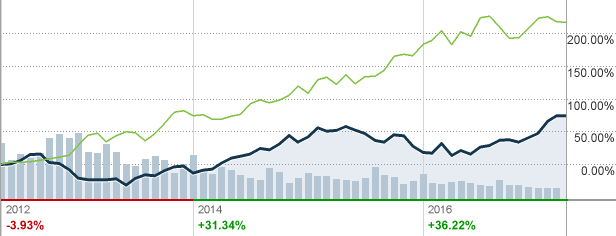
\includegraphics[width=1\textwidth]{apple-chart-5yr}
    \caption{Apple (blue) vs NASDAQ (green) for 5 years~\cite{cnnapple}}
\end{figure}

\newpage

\section{Discussion of Chart}
In the figures found on the previous page, you will notice that I chose to
compare Apple to the NASDAQ for the past 3 months, year, and 5 years. Firstly,
my reasoning for choose NASDAQ was simple; I felt as though it would give a
good visual as to how the market as a whole was doing. Secondly, I selected
multiple graphs so that I could analyze the company for longer than just the
required period; not to mention the \emph{Financial Performance} section has to
do with the past 5 years. Now that the preliminaries are out of the way, let the
discussion begin!

While looking at the graphs, one would notice that Apple seems to be doing quite
poor in comparison to the NASDAQ; except for the past 2 months (Feb. through
Apr.). For the past years, Apple has been dancing around the NASDAQ, as seen in
Figure 2. During spring-summer months, Apple tends to do poorly because they
don't have anything huge being released. iPhones tend to be released in
September and, as we saw earlier, is their biggest seller. This would explain
how in Figure 2, Apple jumps up to about even with the NASDAQ. The new iPhone
would then ride the company through Christmas and into the new year. This
doesn't explain why they are 20\% above the NASDAQ from February until
now. Well, it looks as though the company had it's best holiday quarter ever in
2016~\cite{fool}. Also according to The Motley Fools, ``their fast-growing
service segment ... has expanded to nearly 10\% of sales, and soaring demand for
apps pushed its high-margin revenue.'' This very well could explain that large
jump, although, I'm not sure if I believe it or not.

The last thing to discuss is the company's 5 year graph. In 2012, Apple was
about fair with the NASDAQ. Then the NASDAQ started to move away, and never
crossing paths again until this year. I found this rather interesting but I
believe that the reasoning for this is that Apple has a safety net. The company,
although very intuitive, doesn't make extreme changes on their
products.\footnote{Besides them removing the 3.5mm headset jack on their newest
  model iPhone.} This gives the customer as sense of home, even when they get a
new device. While they are doing that, the market is trying all sorts of new
things. Since the NASDAQ doesn't solely rely on Apple, it might have to do with
other companies making more galvanizing devices that caused the NASDAQ to leave
Apple in the dust.

\section{Financial Performance}
Most of the information I will be discussing in this section can be found in
Appendix A (Balance Sheet), which are sections from Apple's balance sheet. They
contain the past 5 years. Going right down the line, you will find the assets
table first. The very first thing to note is that 2016 seems to have the biggest
numbers in almost all the categories; some even being significantly larger. For
example, their total current assets is up from 2015 by about 17,491 million,
total assets are up 31,207 million, and cash/equivalents are up 25,554
million. There don't seem to be any major decreases, which is good. There are
any major drops, except the drop in other current assets by 6,502
million. Overall, this part of the balance sheet looks good and points the
company toward a successful direction.

Looking at the next piece of the balance sheet is the liabilities. The only
thing that I'm going to note is that the total liabilities seem to be increasing
with time. This isn't necessarily a bad thing, but it isn't necessarily a good
thing either. Luckily, their total assets is significantly greater than their
total liabilities. So far the company seems to be holding up well on their
balance sheet. Let's look into the income and cash flow statements.

The income statement is found in Appendix B (Income Statement). The very first
thing I noticed was that 2016 dropped by about 10,000 million in almost every
category. In fact, the sales dropped by about 15,000 million. Another
interesting thing to note is that 2015 has the highest numbers for all the years
listed. Luckily the cost of goods also dropped as well, saving the company some
money. The numbers dropped, but they didn't drop below any previous year, which
is good. Overall, it's bad that it dropped, but nothing too scary yet. The cash
flow statement, found in Appendix C (Cash Flow Statement), supports the same
claim, for the most part. It seems as though they increased the number of
operating activities\footnote{This could be because of their iPhone recycling
  campaign, if so, that's a warm fuzzy to consider.} and dropped
investments. In this case, some of the values dropped below previous years,
but, yet again, this isn't something to worry about too much. Overall, I believe
that the company is growing, despite having a couple small set backs. I believe
this because the company's numbers are still high and haven't dropped too
low. However, it's still very important that they keep it up or they could be in
trouble.

\newpage

\section{Performance Ratios}


\section{Positives \& Negatives}
Pros and cons

\section{Non-Financial Concerns}
Non-free software!! Spying!!

\section{Competition}
Microsoft, Google, Amazon, Samsung

\section{Other Information}
Who cares

\section{Conclusion}
Please be over.

\section{Required Documents}
Balance Sheet and Income Statement

\newpage

\appendix

\section{Balance Sheet}
\begin{figure}[!htb]
  \centering
  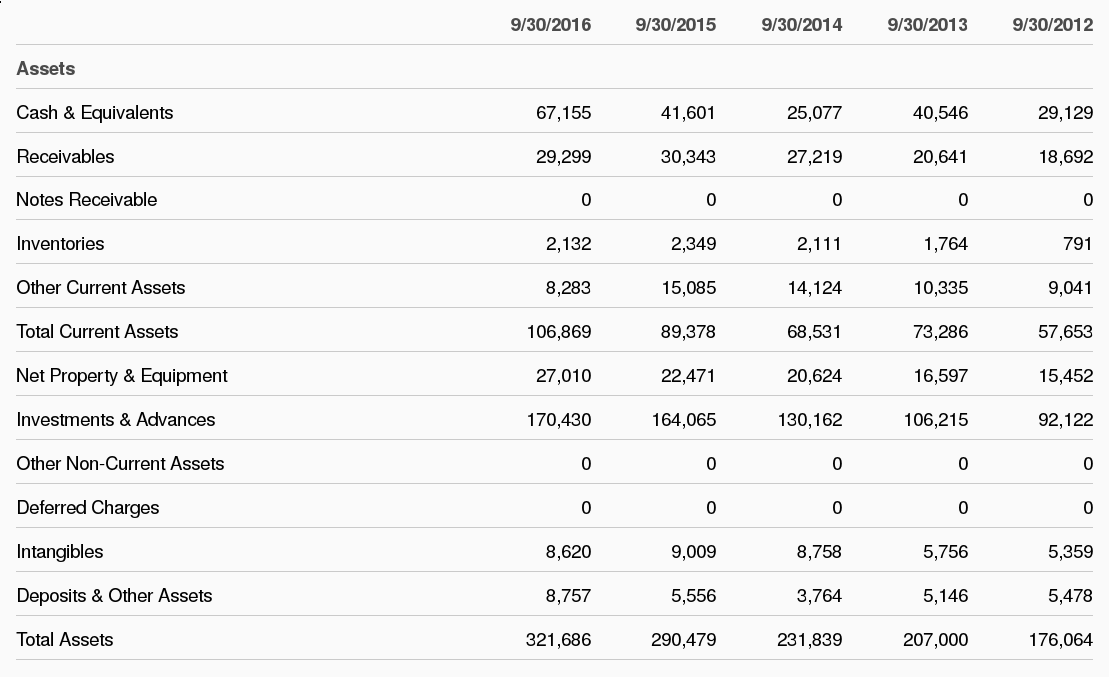
\includegraphics[width=1\textwidth]{assets}
    \caption{Assets. All values in millions except per share data~\cite{zacks-bal}}
\end{figure}

\begin{figure}[!htb]
  \centering
  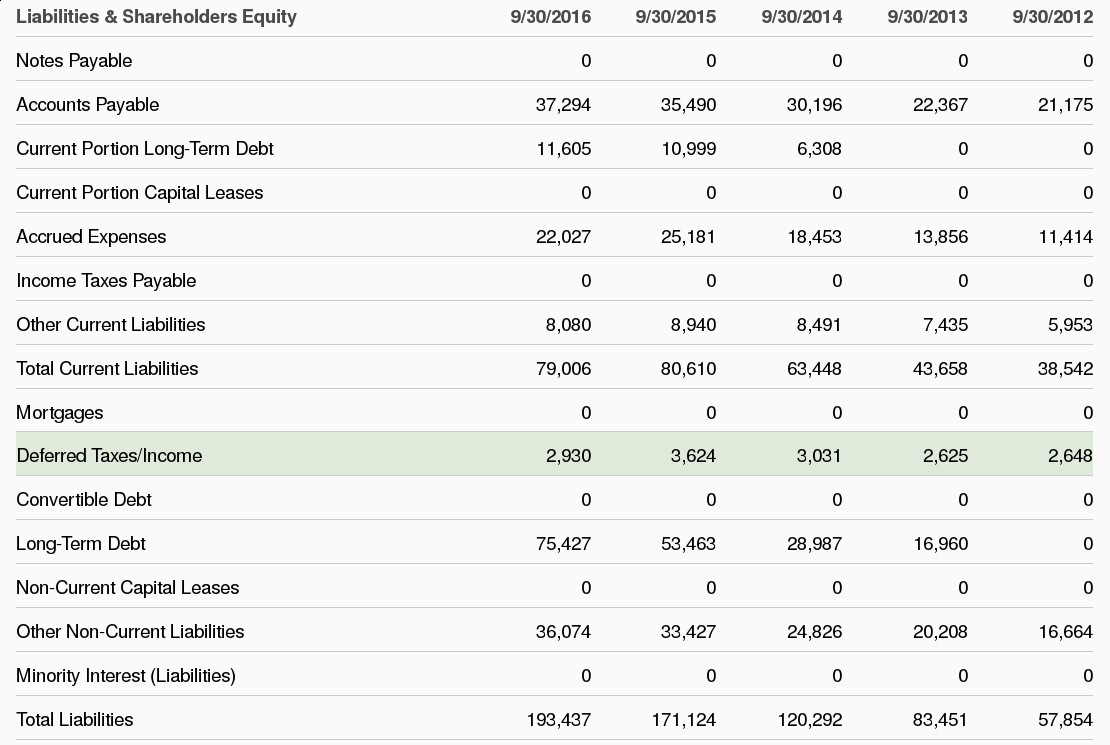
\includegraphics[width=1\textwidth]{liabilities}
    \caption{Liabilities \& shareholder equity. All values in millions except
      per share data~\cite{zacks-bal}}
\end{figure}

\begin{figure}[!htb]
  \centering
  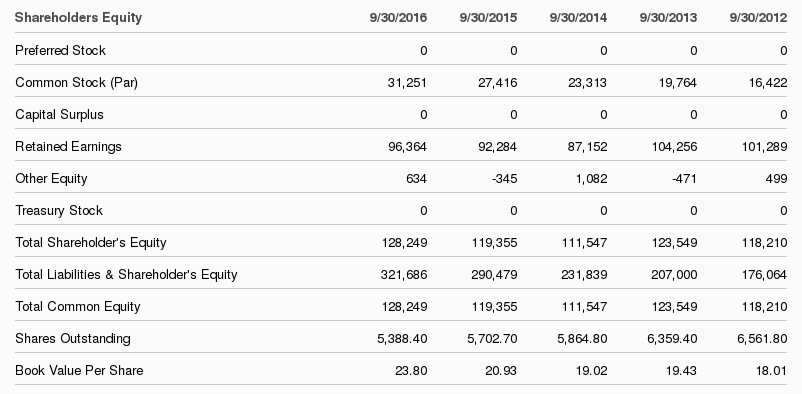
\includegraphics[width=1\textwidth]{shareholder}
    \caption{Shareholder equity. All values in millions except per share
      data~\cite{zacks-bal}}
\end{figure}

\section{Income Statement}
\begin{figure}[!htb]
  \centering
  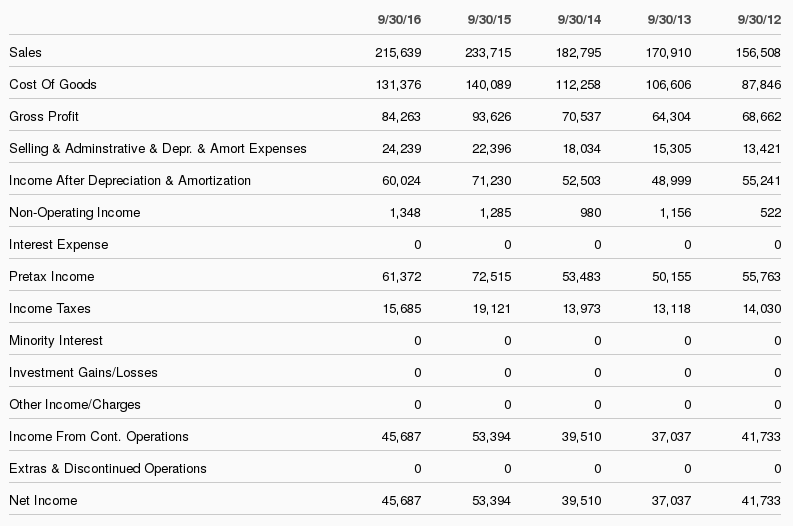
\includegraphics[width=1\textwidth]{income}
    \caption{Income statement. All values in millions except per share
      data~\cite{zacks-income}}
\end{figure}

\section{Cash Flow Statement}
\begin{figure}[!htb]
  \centering
  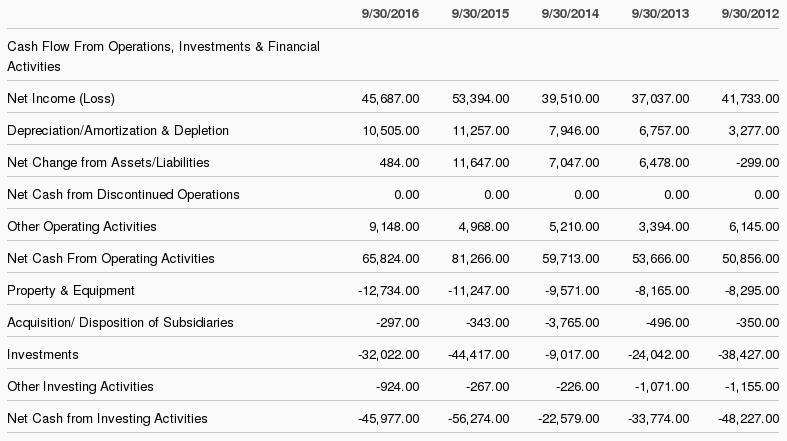
\includegraphics[width=1\textwidth]{cash-flow}
    \caption{Cash flow statement. All values in millions except per share
      data~\cite{zacks-cash}}
\end{figure}

\printbibliography[
heading=bibintoc,
title={Resources}
]

\end{document}
